\documentclass[]{report}

\usepackage[T1]{fontenc}
\usepackage[urw-garamond]{mathdesign}
\usepackage{garamondx}
\usepackage{amsmath, amsthm, amsfonts}
\usepackage[a4paper, total={4in, 8in}]{geometry}
\usepackage{tikz-cd} % used to draw commutative diagrams
\usepackage{graphicx}
\usepackage{hyperref}
\usepackage{mathtools}

% user defined commands go here
\newtheorem{theorem}{Theorem}[section]
\newtheorem{prop}[theorem]{Proposition}
\newtheorem{corollary}{Corollary}[theorem]
\newtheorem{lemma}[theorem]{Lemma}
\newtheorem{defn}[theorem]{Definition}
\newtheorem{examples}[theorem]{Example}
\newtheorem{exercise}[theorem]{Exercise}

\DeclareMathOperator\Spec{Spec}
\DeclareMathOperator\Max{Max}
\DeclareMathOperator\Ker{Ker}
\DeclareMathOperator\Coker{Coker}
\renewcommand{\qedsymbol}{$\blacksquare$}
\newcommand\byS{S^{-1}}
\newcommand\mfk[1]{\mathfrak{#1}}
\newcommand\p{\mathfrak{p}}

\begin{document}

\title{
    Introduction to Commutative Algebra: \\
    
    \large and affine algebraic varieties}
\author{Amal M}
\date{\today}
\maketitle

\begin{abstract}

    The motivation for the study of algebraic geometry is how algebraic objects (rings of rational functions) are associated with varieties (zeros of polynomials). This subject florished during the second half of the twentieth century. Algebraic geometry allows us to study the geometry arising from algebraic objects. Core to the deeper understanding of this subject is an understanding of the subject of commutative algebra which studies commutative rings and their ideals and modules. The purpose of the present project is to gain an understanding of commutative algebra through solving exercises from Atiyah-MacDonald's book, Introduction to Commutative Algebra. The reading project comprised of the study of the theory of rings and modules, their tensor product and exact sequences of rings and modules. The project concluded with a proof of the Going-Up Theorem.

\end{abstract}

\tableofcontents
\newpage

\chapter{Introduction}

The purpose of the current project is to give an understanding 
to the reader of how commutative algebra is used to define the basic
objects of algebraic geometry. Algebraic Geometry is the study of
the geometric properties of the solution set of polynomial equations
in arbitary variables. For this purpose it is useful to confine the 
discussion to algebraically closed fields $k$ and the polynomial ring
$k[x_1,\cdots,x_n]$. Since $k$ is a field, $k^n$ is a vector field for all $n>1$. An \textit{affine space} is a special vector space where we do not associate a unique vector to a point, that is, we do not consider each point of the vector space as a vector from a unique origin to the point. Instead we think only about vectors from any $a$ to any other point $b$ as translation vectors. Thus, in an \textit{affine space} we have dispensed with the concept of an origin. 

The \textit{affine n-space} over the algebraically closed field $k$ is the vector space $k^n$, denoted by $\mathbb{A}^n_k$.

\begin{defn} The algebraic variety \cite{vakil145} in the affine space $\mathbb{A}^n_k$ of a set $S$ of polynomials $f\in k[x_1,\cdots, x_n]$, is a subset $V(S)\subseteq \mathbb{A}^n_k$ cut out by the set of mutual zeros of all the polynomials in the set $S$.  
    $$V(S) = \{x = (x_1,\cdots,x_n) \in \mathbb{A}^n_k : f(x) = 0 \text{ for all } f \in S\}.$$
\end{defn}

The affine variety is not the only example of a variety. The projective variety defined over projective spaces $\mathbb{P}^n_k$ is another example of an algebraic variety.

The solution set or \textit{locus} of solutions of polynomials of degree one are discrete points in $k$. But over $k^2$ the \textit{locus} are curves or intersections of curves. For example, the solution of the elliptic curve given by the polynomial equation in $\mathbb{R}[x,y]$ in $\mathbb{R}^2$  
    $$y^2 = x^3 - 3x + 5$$
    is a curve (Fig 1.).

    Naturally, the question arises: \textit{what does the solution set of a set of polynomials in $k^3$ look like? What about $k^n$?} which is the same as asking \textit{what does an affine algebraic variety in $\mathbb{A}^n_k$ look like?} In general it is an intersection of a collection of affine algebraic hypersurface of $n-1$ dimension each defined by one of the polynomials.

    We may go further. \textit{What is the topology of the affine algebraic variety?} There is no one single way to define a topology on an affine algebraic variety. But the first topology we shall introduce is called the \textit{Zariski Topology}.

    Once we have an affine algebraic variety we may define functions on them and we may define functions from one algebraic variety to another. Such functions are called \textit{polynomial functions}. Thus we start to do the usual mathematical \textit{shtick} on affine varieties.

    To answer the proposed questions we need to know the properties of an affine algebraic varieties. For example: \textit{what is so algebraic about an affine algebraic variety?} We will see that the answer to this question is the fact that we may consider every \textit{affine algebraic variety} to be some \textit{finitely generated nilpotent-free $k$-algebra $A$}. To know what each of these terms means we first need some commutative algebra. The purpose of this article is to explain these terms and give a brief introduction to Algebraic Geometry focusing only on affine algebraic varieties.

    The exposition is based on the knowledge gained after spending many hours working out the exercises contained in \cite{atiyah1}. I would advise anyone thinking about learning algebraic geometry to start there and work out those exercises themselves.  

    We divide the article into four sections. In the first section we introduce the \textit{prime spectrum} of a ring $A$, $X = \Spec(A)$ by which we denote the set of all prime ideals of $A$. We endow this space $X$ with a topology called \textit{the Zariski Topology}.

    In the next section, we introduce \textit{modules}, which are a sort of generalised vector spaces and \textit{algebras}, which are modules on rings, and we define the tensor product on a collection of such \textit{modules}. Then we discuss a particular sort of structure that can be given to a collection of modules called \textit{the direct limit}.

    In the third section we introduce the \textit{rings of fractions} of modules and the concept of \textit{localization} which we use in the formulation of a sort of structure called \textit{presheaf} and \textit{sheaf} which is a method to talk about a collection of open sets on a topological space. We also introduce the \textit{constructible topology} and the precise condition under which this topology is equivalent to the \textit{Zariski Topology} on $\Spec(A)$. 

    In the final section we introduce integral dependence, that is elements of rings that are integral over a subring and discuss the proof of the Going-Up Theorem.

    % Start by giving an overview of the table of content

\begin{figure}
  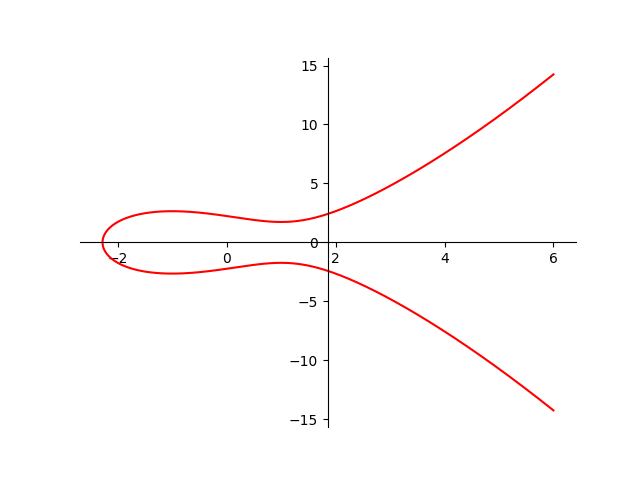
\includegraphics[width=\linewidth]{img/ell_curv1.png}
  \caption{Fig 1.}
  \label{fig:ell_curv1}
\end{figure}

\chapter {The Zariski Topology}

In commutative algebra what we generally call a \textit{ring} is a commutative ring with unity, i.e, $1\in A$. So from now on, when we say ring we mean a set $A$ with two binary operations on it's elements $a + b \text{ and } a\dot b$, for all $a,b\in A$ such that A is an abelian group with respect to addition and multipication is associative as well as distributive over addition.

A \textit{unit} in a ring $A$ is an element $x\in A$ such that there is another element $y\in A$ so that $xy = 1$. A ring in which every element is a \textit{unit} is called a \textit{field}. 

An element $x\in A$ is a \textit{nilpotent} element if $x^n = 0$ for some $n>0$. An element $x$ is an \textit{idempotent} element if $x^2 = x$. 

If we are given a group $G$ and a normal subgroup $N$, the quotient group $G/N$ is also a group. Similarily if $f: G \rightarrow G'$ is a group homomorphim, the kernel of $f$, $\Ker(f)$ is a normal subgroup in $G$. 

In the case of rings the role of a normal subgroup is played by subsets of $A$ called \textit{ideals}. Quotienting by an ideal gives another ring and all kernals of ring homomorphims are ideals as well.

\begin{defn}
    A subset $\mathfrak{a} \subseteq A$ is called an \textit{ideal} of $A$ if $\mathfrak{a}$ is an additive subgroup and it has the property, $y\in \mathfrak{a}$ and $x\in A$ implies $xy\in \mathfrak{a}$.
\end{defn}

 There are two special cases of \textit{ideals} that we are interested in, the \textit{prime ideal} and the \textit{maximal ideal}. A \textit{prime ideal} of $A$  is an ideal $\mathfrak{p}$ of $A$ with the property that $xy\in \mathfrak{p} \implies x \in \mathfrak{p} \text{ or } y\in \mathfrak{p}$. An ideal $\mathfrak{m}$ is a \textit{maximal ideal} if $\mathfrak{m} \neq (1)$ and if there is no ideal $\mathfrak{a}$ such that $\mathfrak{m\subset a\subset} (1)$. 

\begin{prop}
    \begin{enumerate}
        \item $\mathfrak{p}$ is a \textit{prime ideal} if and only if $A/\mathfrak{p}$ is an \textit{integral domain }. 
        \item $\mathfrak{m}$ is a \textit{maximal ideal} if and only if $A/\mathfrak{m}$ is a field.
    \end{enumerate}
\end{prop}
\begin{proof}
    \begin{enumerate}
        \item Assume that $\mfk{p}$ is a prime ideal and let $\bar{x} \bar{y} = \bar{xy} = 0$, where $\bar{x}, \bar{y} \in A/\mfk{p}$. We have, $xy \in \mfk{p}$. Hence $x \text{ or } y \in \mfk{p}$. Which means $\bar{x} = 0 \text{ or } \bar{y} = 0$. Therefore $A/\mfk{p}$ is an \textit{integral domain}.

            Conversely, let $A/\mfk{p}$ be an \textit{integral domain}. We have $\bar{x}\bar{y} = 0$ implies $\bar{x} = 0 \text{ or } \bar{y} = 0$. That means $xy \in \mfk{p}$ implies $x \text{ or } y \in \mfk{p}$. So $\mfk{p}$ is \textit{prime}.

        \item Assume that $\mfk{m}$ is a \textit{maximal ideal} of $A$. Let $\mfk{a}$ be an ideal of $A/\mfk{m}$ not equal to $(0) \text{ or } (1)$. Since there is a one-to-one correspondence between ideals of $A/\mfk{m}$ and the ideal of $A$ containing $\mfk{m}$, this would mean that there exists an ideal $\mfk{b} \subseteq A$ such that $\mfk{b} = \phi^{-1}(\mfk{a})$ so that $\mfk{b} \supset \mfk{m}$ which is a contradiction since $\mfk{m}$ is maximal. Therefore $A/\mfk{m}$ is a field.

            Conversely, let $A/\mfk{m}$ be a field. Then the only ideal of $A$ which contains $\mfk{m}$ is the whole ring $A$ since in $A/\mfk{m}$, the corresponding ideal can only be $(1)$. Hence $\mfk{m}$ is a \textit{maximal ideal}.
    \end{enumerate}
\end{proof}

Therefore every \textit{maximal ideal} is a \textit{prime ideal} but the converse is not true in general. The reason prime ideals and maximal ideals are so important is because they have "nice" properties when we transport them across ring homomorphims. For example given a ring homomorphim $f:A\rightarrow B$ and a prime ideal $\mathfrak{q}\subset B$ the set $f^{-1}(\mathfrak{q})$ is a prime ideal  $\mathfrak{p}\subset A$. 
\begin{proof}
    Let $xy \in f^{-1}(\mathfrak{q})$. Then $f(xy) = f(x).f(y) \in \mathfrak{q}$. Since $\mathfrak{q}$ is \textit{prime}, either $f(x) \in \mathfrak{q} \text{ or } f(y) \in \mathfrak{q}$. Therefore we have either $x \text{ or } y \in f^{-1}(\mathfrak{q})$.
\end{proof}


This result will be useful later on.

A ring with just one \textit{maximal} ideal $\mathfrak{m}$ is called a \textit{local ring}. The quotient ring $k = A/\mathfrak{m}$ which is a field, is called the \textit{residue field} of $A$. 

\begin{defn}
    The radical of an ideal $\mathfrak{a}\subset A$ is another ideal 
    $$r(\mathfrak{a}) = \{x\in A: x^n\in \mathfrak{a} \text{ for some } n>0\}$$
\end{defn}

We can show that the \textit{radical} of an ideal is the intersection of all prime ideals that contain that ideal \cite{atiyah1}. If $x$ is an element of $\mathfrak{a}$ and if $x$ is any power of an element then that element belongs to the \textit{radical}. So the \textit{radical} is a way to associate elements related to $\mathfrak{a}$ by it's power. That is, if $f^n\in \mathfrak{a}$ then by definition of an ideal all the powers of $f$ higher than $n$ also belongs to $\mathfrak{a}$, the \textit{radical} ideal includes \textit{lower powers} of $f$ such as $f^{n-2}, f^{n-5}$ and so on. So we can have all powers of $f$ in $r(\mathfrak{a})$ if just one power of $f$ is in $\mathfrak{a}$. 

We just need to define one more concept before we can move on to define the \textit{prime spectrum} of a ring. The set of all nilpotent elements in a ring is called the \textit{nilradical} of $A$ and is denoted by $\mathfrak{N}$.

\begin{prop}
    The set $\mathfrak{N}$ of all nilpotent elements in a ring A is an ideal and $A/\mathfrak{N}$ has no nilpotent element $\neq 0$. \cite{atiyah1}
\end{prop}

The \textit{nilradical} of a ring $A$ has the property that it is equal to the intersection of all the prime ideals of $A$. \textit{What is the intersection of all maximal ideals of $A$?}. The answer is called the \textit{Jacobson ideal} of $A$ denoted by $\mathfrak{R}$. It has the following property

\begin{prop}
    $x\in \mathfrak{R} \Leftrightarrow 1-xy$ is a unit in A for all $y\in A$. \cite{atiyah1}
\end{prop}

\section{Prime Spectrum}

The \textit{prime spectrum} of a ring is the set of all \textit{prime} ideals of the ring $A$ and we denote it by $X = \Spec(A)$. To this "set" of elements we associate a topology called the \textit{Zariski Topology} therefore making $\Spec(A)$ a topological space. Since we will consider $\Spec(A)$ to be a space, from now on it's convenient to talk about the elements of $\Spec(A)$ as points, i.e., each \textit{prime ideal} $\mathfrak{p}_x \in \Spec(A)$ is a point which we denote by $x$. We use the subscript notation to fix the correspondence between the \textit{prime ideal} $\mathfrak{p}_x$ when thinking of $X$ as a set of ideal and the point $x$ when thinking of $X$ as a space. Note that this is just convention and $x$ and $\mathfrak{p}_x$ are really just two notations for the same object, i.e, an element of the set $\Spec(A)$.

A topology on a space can be axiomatically defined using just the closed sets. That is we need only satisfy these axioms
\begin{enumerate}
    \item The sets $\varnothing$ and $X$ are closed. 
    \item Arbitary intersection of closed sets are closed. 
    \item Finite union of closed sets are closed.
\end{enumerate}

The \textit{Zariski Topology} is the topology on $\Spec(A)$ for which the subsets of $\Spec(A)$
$$V(E) = \{\mathfrak{p}\in \Spec(A): \text{ all prime ideals } \mathfrak{p} \text{ containing } E\}$$
 for each subset $E$ of $A$, satisfies the axioms for closed sets. 
\begin{proof}
\begin{enumerate}
    \item Every ideal contains $(0)$. Therefore $V(0) = X$.

        If a \textit{prime ideal} $\mathfrak{p}$ contains $1$ then every element of $A$ belongs in $\mathfrak{p}$ and so $\mathfrak{p} = A$, the entire ring. Since $A$ is not considered a \textit{prime ideal}, $V(1) = \varnothing$. 
        
        Therefore $X$ and the empty set $\varnothing$ are both closed sets.
    \item Let $(E_i)_{i \in I}$ be a collection of subsets of $A$. Each $V(E_i)$ is a closed set. We show that 
        $$V(\bigcup_{i \in I} E_i) = \bigcap_{i \in I} V(E_i).$$

        Let $\mathfrak{p} \in V(\bigcup_{i \in I} E_i), \mathfrak{p}$ is a prime ideal. Then $\bigcup_{i \in I} E_i \subseteq \mathfrak{p}$. Which means that for each $i$, $E_i \subseteq \mathfrak{p}$. Hence $\mathfrak{p} \in V(E_i), \forall i \in I$, i.e, $\mathfrak{p} \in \bigcap_{i \in I} V(E_i)$. So we have our first inclusion
        $$V(\bigcup_{i \in I} E_i) \subseteq \bigcap_{i \in I} V(E_i).$$
        
        Conversely, let $\mathfrak{p} \in \bigcap_{i \in I} V(E_i), \mathfrak{p}$ is a prime ideal. Then $\mathfrak{p} \in V(E_i), \forall i \in I$. Which means $E_i \subseteq \mathfrak{p}, \forall i \in I$. Hence $\bigcup_{i \in I} E_i \subseteq \mathfrak{p}$and so $\mathfrak{p} \in V(\bigcup_{i \in I} E_i)$. So we get our second inclusion
        $$\bigcap_{i \in I} V(E_i) \subseteq V(\bigcup_{i \in I} E_i),$$
        therefore
        $$V(\bigcup_{i \in I} E_i) = \bigcap_{i \in I} V(E_i).$$

        In the \textit{Zariski Topology} the closed sets are only those subsets of $X$ of the form $V(E)$ for some subset $E$ of $A$. Therefore this equation states precisely that the intersection of arbitary closed sets is a closed set.
    \item Let $E \subseteq A$ and let $\mathfrak{a}$ be the ideal generated by $E$ in $A$. If $\mathfrak{p} \in V(E)$ then $\mathfrak{p}$ is a prime ideal containing $E$. As $\mathfrak{a}$ is generated by $E$ it is also contained in $\mathfrak{p}$, i.e., $\mathfrak{p} \in V(\mathfrak{a})$. Hence $V(E) \subseteq V(\mathfrak{a})$.

        Conversely, let $\mathfrak{p} \in V(\mathfrak{a})$, $\mathfrak{p}$ is a prime ideal containing $\mathfrak{a}$. But $\mathfrak{a}$ is generted by $E$, hence $E \subseteq \mathfrak{a}$. So $E \subseteq \mathfrak{p}$ as well. Therefore $\mathfrak{p} \in V(E)$. Hence we have the reverse inclusion $V(\mathfrak{a}) \subseteq V(E)$. Therefore we have
        $$V(E) = V(\mathfrak{a}).$$

        We shall now show that $V(\mathfrak{a} \cap \mathfrak{b}) = V(\mathfrak{ab})$. Let $\mathfrak{p} \in V(\mathfrak{a} \cap \mathfrak{p}), \mathfrak{p}$ is a prime ideal. So $\mathfrak{a} \cap \mathfrak{b} \subseteq \mathfrak{p}$. But we also have the identity $\mathfrak{ab} \subseteq \mathfrak{a} \cap \mathfrak{b}$. So $\mathfrak{ab} \subseteq \mathfrak{p}$, which means that $\mathfrak{ab} \subseteq V(\mathfrak{p})$. So $\mathfrak{p} \in V(\mathfrak{ab})$. Therefore we have the inclusion $V(\mathfrak{a}) \cap \mathfrak{b}) \subseteq V(\mathfrak{ab})$.

        Conversely, let $\mathfrak{p} \in V(\mathfrak{ab}), \mathfrak{p}$ is a prime ideal so that we have $\mathfrak{ab} \subseteq \mathfrak{p}$. Suppose $x \in \mathfrak{a} \cap \mathfrak{b}$. Then $x \in \mathfrak{a} \text{ and } x \in \mathfrak{b}$. Which means $x^2 \in \mathfrak{ab} \subseteq \mathfrak{p}$. As $\mathfrak{p}$ is prime we have $x \in \mathfrak{p}$. Hence $\mathfrak{a} \cap \mathfrak{b} \subseteq \mathfrak{p}$. So $\mathfrak{p} \in V(\mathfrak{a} \cap \mathfrak{b})$. Therefore we have the inclusion $V(\mathfrak{ab}) \subseteq V(\mathfrak{a} \cap \mathfrak{b})$. So we have
        $$V(\mathfrak{ab} = V(\mathfrak{a} \cap \mathfrak{b}).$$


        Now, let $(E_i)_{i \in I}$ be a finite family of subsets of $A$. We have $V(E_i) = V(\mathfrak{a}_i), \forall i \in I$. By induction, using the formula above 
        $$\bigcup_{i \in I} V(E_i) = \bigcup_{i \in I} V(\mathfrak{a}_i) = V(\prod_{i \in I} \mathfrak{a}_i).$$
        Since so we see that the union of finitely many closed set is also closed. So we have shown that $\Spec(A)$ satisfies the \textit{Zariski Topology}.
\end{enumerate}
\end{proof}

    This is not the only topology on $\Spec(A)$ we will discuss another such topology, the \textit{constructible topology}, later on. But for now we focus on the properties of the \textit{Zariski Topology}.

    The sets $X_f = X - V(f)$ are open sets in $X$ for each $f\in A$ since each $V(f)$ is closed. The family of such sets, $\{X_f\}_{f\in A}$ is the basis (Ex 17) of the \textit{Zariski Topology} and we call them the \textit{basic open sets} of $X$.

\begin{proof}
    If $\{X_f\}_{f \in A}$ is a basis of the \textit{Zariski Topology} then it must satisfy two conditions
    \begin{enumerate}
        \item $\{X_f\}_{f \in A}$, covers $X = \Spec(A)$.
        \item If $X_f, X_f$ are base elements then if $x \in X_f \cap X_g$ then there exists an $X_h$ such that $x \in X_h$ and $X_h \subseteq X_f \cap X_g$.     \end{enumerate}

    If $\mathfrak{p}$ is a prime ideal $1 \not \in \mathfrak{p}$  implies $\mathfrak{p} \in X_1$. Which proves (1).

    We know that $X_f \cap X_g = fg$. If $x \in X_f \cap X_g$ then $x \in X_{fg}$ which belongs to the basis set. So (2) is satisfied. Hence $\{X_f\}_{f \in A}$ is a basis for $X = \Spec(A)$ endowed with the \textit{Zariski Topology}.

\end{proof}

$X$ is \textit{quasi-compact}. That is every open covering of $X$ has a finite sub-cover.
\begin{proof}
    Let $\{X_{f_i}\}_{i \in I}$ be a covering of $X$ by basic open sets, $X = \bigcup_{i \in I} X_{f_i}$. It's easy to see that any open open covering of $X$ can be turned into a covering involving only \textit{basic open set}. Just replace each open sets by the open sets in the basis whose union it is composed off. 

    We have $X_{f_i} = X - V(f_i), \forall i \in I$. Let $E = \{f_i : i \in I\}$, and $\mathfrak{a}$ is the ideal generated by $E$so that $V(\mathfrak{a} = V(E)$. Assume that $\mathfrak{p}$ is a prime ideal such that $f_i \in \mathfrak{p} \forall i \in I$ then, $\mathfrak{p} \not \in X_{f_i}, \forall i \in I$. Which means $\mathfrak{p} \not \in \bigcup_{i \in I} X_{f_i}$. But $\bigcup_{i \in I} X_{f_i} = X$ implies that $\mathfrak{p} \not \in X$, which is a contradiction. Which implies there exists no prime ideal $\mathfrak{p}$ such that $f_i \in \mathfrak{p}, \forall i \in I$. Which means that $V(\mathfrak{a}) = \varnothing$. Therefore $\mathfrak{a} = (1)$.

    Since $1 \in \mathfrak{a}$ then it must be representable as a finite sum  by definition, i.e., $1 = \sum_{i \in J} g_i f_i$, where $J$ is a finite subset of $I$. Which means that $\mathfrak{a} = (1) = (f_i)_{i \in J}$.
    
    Hence $\varnothing = V(1) = V(\mathfrak{a}) = V(E) = V(E')$ where $E'$ is the subset of $E$ containing only finitley many $f_i$, i.e., $i \in J$. 

    If $\mathfrak{p} \in X$ then $\mathfrak{p} \not \in V(\mathfrak{a}) = V(E')$. Which means $E' \not \subseteq \mathfrak{p}$. Therefore for some $i \in J$, there exists $f_i \in E'$ such that $f_i \not \in \mathfrak{p}$ which is same as $\mathfrak{p} \in X_{f_i}$.

    Hence $X$ is covered by a finite covering.
\end{proof}

    Which is exactly the same as \textit{compactness} in regular topology. For some reason Algebraic Geometers do not use the term \textit{compactness} to mean just the condition \textit{every open cover has a finite subcover}. But instead a space is \textit{compact} if it is also Hausdorff as well as \textit{quasi-compact}. This is because every $\Spec(A)$ has the usual property of having a finite subcover for an open covering. So just calling it \textit{compact} is a waste of a perfectly good word that can be used for something more significant. 

    We find that every open set $X_f$ is quasi-compact as well every finite union of sets $X_f$. Indeed we have that a subset of $X$ is quasi-compact if and only if it is a union of finitely many open sets $X_f$.

    A singleton set $\{x\}$ in the Zariski Topology is closed if and only if $\mathfrak{p}_x$ is maximal.
\begin{proof}
    If a set $B \subset \Spec(A)$ is closed in the Zariski Topology then there exists a set $E \subseteq A$ such that $B = V(E)$. If $\{x\}$ is closed then there exists some $E$ such that $x$ is the only element of $V(E)$. That means $x$ is the only prime ideal such that $E \subseteq \mathfrak{p}_x$. If $\mathfrak{p}_y$ is another prime ideal such that $E \subseteq \mathfrak{p}_x \subseteq \mathfrak{p}_y$ then $x = y$. Hence $\mathfrak{p}_x$ is maximal.
\end{proof}

    Now would be a good time to see some examples of the \textit{prime spectrum} of some well known rings such as $\mathbb{Z, R, C}[x]$ and $\mathbb{Z}[x]$ (Ex 16).



\section{Maximal Spectrum}

The \textit{maximal spectrum} of a ring is the set of all \textit{maximal} ideals of the ring. It is denoted by $\Max(A)$. The \textit{maximal spectrum} is a subset of the \textit{prime spectrum} $\Spec(A)$. We can quickly give a concrete example for a \textit{maximal spectrum}.

Let $X$ be a compact Hausdorff space and let $C(X)$ be the ring of all real valued continuous functions on $X$. Define
$$\mathfrak{m}_x = \{f\in C(X): f(x) = 0\}$$
Then $\mathfrak{m}_x$ is an ideal and furthermore it is a maximal ideal since if we define a function $\phi_x: C(X) \rightarrow \mathbb{R}$ as the mapping $f\mapsto f(x)$ then the kernel of the map is $\mathfrak{m}_x$. 

Let $\hat{X} = \Max(A)$ we can define a mapping $\mu: X\rightarrow \hat{X}$ by $x\mapsto \mathfrak{m}_x $. By Ex 26.i $\mu$ is surjective and by Ex 26.ii it is injective. Let $f\in C(X)$ and define
$$U_f = \{x\in X:f(x) = 0\}$$
$$\hat{U}_f = \{\mathfrak{m}\in \hat{X}:f\not\in \mathfrak{m}\}$$
We can show that $\mu(U_f) = \hat{U}_f$ (Ex 27.iii). So $\mu$ sends the basis of $X$ the basis of $\hat{X}$ and so $\mu$ is a homeomorphism.

We have just show that given only the ring of functions on a compact Hausdorff space $X$ we can reconstruct the underlying space by just looking at the \textit{maximal specttrum} of the ring.


\section{Affine Algebraic Varieties}

Given a set $S$ of polynomial in $k[x_1,\cdots,x_n]$ we have defined the \textit{affine algebraic variety} on $S$ as the subset $V(S)$ of the affine space $\mathbb{A}^n_k$.
$$V(S) = \{x = (x_1,\cdots,x_n) \in \mathbb{A}^n_k : f(x) = 0 \text{ for all } f \in S\}.$$

Given a subset $X$ of the affine space we define the \textit{ideal of the variety} $X$ to be the set of polynomials $g\in k[x_1,\cdots,x_n]$ that vanish on $X$. It is denoted by $I(X)$.
$$I(X) = \{g\in k[x_1,\cdots,x_n]: g(x) = 0, \forall x\in X\}$$

If $f,g$ are two polynomials in $I(X)$ then $f+g$ is also a member of $I(X)$ since both $f$ and $g$ vanish on $X$. Hence $I(X)$ is an additive subgroup of $k[x_1, \cdots, x_n]$. Given $g \in I(X)$ and $f \in k[x_1, \cdots, x_n]$ then $(fg)(x) = 0, \forall x \in X$ as $g(x) = 0$ on $X$. So $fg \in I(X)$ whenever $g \in I(X)$. Therefore $I(X)$ is a ideal in $k[x_1, \cdots, x_n]$.

\begin{defn} 
    The quotient ring
    $P(X) = k[x_1,\cdots,x_n]/I(X)$
    is called the ring of polynomial functions on $X$. 
\end{defn}

If two polynomials $f$ and $g$ are similar in $P(X)$, then $f-g \in I(X)$ that means over $X$, $(f-g)(x) = 0$, i.e., the two polynomials agree in value over $X$. So the polynomial ring contains polynomials which have distinct values over $X$.

\begin{defn}
    Let $\xi_i$ be the image in $P(X)$ of $x_i$, i.e., the coset $x_i + I(X)$. Then the $\xi_i (1\leq i\leq n)$ are called the \textit{coordinate functions} on $X$. $P(X)$ is generated as a $k$-algebra by the \textit{coordinate functions} and it is called the \textit{coordinate ring} or \textit{affine algebra} on $X$.
\end{defn}

By a $k$-algebra we mean a vector space over $k$ with a bilinear product. That is if $A$ is a vector space over $k$, we have a product operation defined on $A$ as
    $$A \times A \rightarrow A.$$


    For each $x\in X$ the ideal $\mathfrak{m}_x$ consiting of $f\in P(X)$ such that $f(x) = 0$ is a maximal ideal. Let $\hat{X} = \Max(P(X))$. We can to show that the mapping $\mu: X \rightarrow \hat{X}$ given by $x\mapsto \mathfrak{m}_x$ is a bijection.

    So far we have seen that the \textit{affine algebraic variety}, $X$ has the \textit{Zariski Topology} and that we can define a ring called the \textit{coordinate ring} $P(X)$ on the variety so that the maximal spectrum of the ring is in bijection with the variety itself. 


\begin{defn}
    Let $f_1,\cdots, f_m$ be $m$ polynomials in $k[x_1,\cdots,x_n]$. We can define a mapping $\phi: k^n\rightarrow k^m$ by $\phi(x) = (f_1(x),\cdots,f_m(x))$. Such a mapping is called a \textit{polynomial mapping}.
\end{defn}


    Let $X,Y$ be affine algebraic varieties in $k^n$ and $k^m$ respectively. A mapping $\phi: X \rightarrow Y$ is a \textit{regular} mapping if $\phi$ is a restriction of a polynomial mapping from $k^n$ to $k^m$.

    If $\eta$ is a polynomial function on $Y$, then $\eta \circ \phi$ is a polynomial function on $X$. So we have a $k$-algebra homomorphim $P(Y) \rightarrow P(X)$ given by $\eta \mapsto \eta \circ \phi$.

\chapter{Tensor Product and Direct Limits}

\begin{defn}
    Let $A$ be a ring. An $A$-\textit{module} is an abelian group $M$ along with a mapping $\mu: A\times M\rightarrow M$, $\mu(a,x)$ denoted by $ax, a\in A, x\in M$ which satisfies the following
\begin{enumerate}
    \item $a(x+y) = ax + ay$
    \item $(a+b)x = ax + bx$
    \item $(ab)x = a(bx)$
    \item $1x = x$, 
 ($\forall a,b \in A, \forall x,y \in M$.)
\end{enumerate}
\end{defn}

We may consider the mapping $\mu: A \times M \rightarrow M$ to be an action of $A$ on $M$.

\begin{defn}
    A \text{module homomorphism} between two modules $M$ and $N$ is a called an $A$-\textit{linear mapping} or an $A$-module homomorphim $f:M\rightarrow N$, if the following two properties are satisfied
\begin{enumerate}
    \item $f(x+y) = f(x) + f(y)$
    \item $f(a.x) = a.f(x)$
\end{enumerate}
\end{defn}

A module $M'$ is called a \textit{submodule} of $M$ if it is a subgroup that is closed under multiplication by elements of $A$. The quotient $M/M'$ is an A-module as well.

\begin{defn}
    Given two modules $M$ and $N$, their direct product is given as the module $M\oplus N$ which is the set of all elements $(x,y) \text{ where } x\in M \text{ and } y\in N$ along with the following two operations 
$$(x_1,y_1) + (x_2,y_2) = (x_1+x_2, y_1+y_2)$$
$$a(x,y) = (ax, ay).$$
\end{defn}

Given an arbitary family of $A$-modules, $(M_i)_{i\in I}$ the direct sum of the family is the sum $\bigoplus_{i\in I} M_i$ is the set of all families $(x_i)_{i\in I}$, $x_i\in M_i$ such that all but finitely many $x_i$ are nonzero.

\section{Exact Sequences}

\begin{defn}
    Given an $A$-module homomorphim $f: M' \rightarrow M$ the cokernel of $f$ is the quotient module $M/f(M')$. This is denoted by $\Coker(f)$.
\end{defn}


A sequence of $A$-modules and $A$-homomorphisms,
$$\cdots \rightarrow M_{i-1} \xrightarrow{f_i} M_i \xrightarrow{f_{i+1}} M_{i+1} \rightarrow \cdots$$ 
is said to be \textit{exact} at $M_i$ if, $\Ker(f_{i+1}) = \text{Im}(f_i)$. The sequence is exact if it is exact at each $M_i$. 

\begin{enumerate}
    \item The sequence $0 \rightarrow M' \xrightarrow{f} M$ is exact if and only if $f$ is injective.
    \item The sequence $M \xrightarrow{g} M'' \rightarrow 0$ is exact if and only if $g$ is surjective. 
    \item The sequence $0 \rightarrow M' \xrightarrow{f} M \xrightarrow{g} M'' \rightarrow 0$ is exact if and only if $f$ is injective and $g$ is surjective and also that $g$ induces an isomorphisms of $\Coker(f) = M/f(M')$ onto $M''$. This sequence called a \textit{short exact sequence}.
\end{enumerate}

\begin{proof}
    \begin{enumerate}
        \item Let $0 \rightarrow M' \xrightarrow{f} M$ be an exact sequence. The image of $0 \rightarrow M'$ is $0$. Hence the kernel of $f: M' \rightarrow M$ is $0$. Therefore $f$ is injective.

            Conversely, let $f$ be injective. $\Ker(f)$ is hence $0$. In that case $\Ker(f)$ is the image of the map $0 \rightarrow M'$. Therefore the sequence is exact.
        \item Let $M \xrightarrow{g} M'' \rightarrow 0$ be an exact sequence. The kernel of $M'' \rightarrow 0$ is the entire module $M''$. Therefore the image of $g$ is $M''$ and so $g$ is surjective.

            Conversely, let $g$ be a surjective mapping. Then the$\text{Im}(g)$ is the module $M''$. But it is also the kernel of $M'' \rightarrow 0$. Therefore the sequence is exact.
        \item Let the sequence be exact. By (1) and (2) $f$ is injective and $g$ is surjective. We also have that $M'' \cong M/\Ker(g)$. Since the sequence is exact $\Ker(g) = \text{Im}(f) = f(M')$. Therefore $M'' \cong M/f(M') = \Coker(f)$. The converse is follows similarily.
    \end{enumerate}
\end{proof}

\section{Tensor Product}

\begin{defn}
    The \textit{tensor product} of two $A$-modules $M$ and $N$ is an $A$-module denoted by $M\otimes N$ which is the set of all linear combination of the pair $x \otimes y$ with coefficients in $A$ along with the following properties for all $x,x' \in M; y, y' \in N \text{ and } a \in A$,
\begin{enumerate}
    \item $(x + x') \otimes y = x \otimes y + x' \otimes y$
    \item $x \otimes (y + y') = x \otimes y + x \otimes y'$
    \item $a.x \otimes y = x \otimes a.y = a(x \otimes y)$
\end{enumerate}
\end{defn}

We see that $0 \otimes x = x\otimes 0 = 0$ as $0.(a\otimes x) = 0$. If $x_i$ generates M and $y_i$ generates N then $x_i \otimes y_i$ generates $M\otimes N$. Let $x\in M$ and $y\in N$ if $M' \subseteq M$ and $N'\subseteq N$ are submodules then $x\otimes y \in M\otimes N$ is not the same as $x\otimes y \in M'\otimes N'$. To be specific the tensor product of A-modules is denoted by $M \otimes_A N$ but if the context is clear we can write $M\otimes N$. The following are some useful properties of \textit{tensor product}.

\begin{prop} 
    Let M,N,P be A-modules. Then there exists unique isomorphisms called the cannonical isomorphisms 
    \begin{enumerate}
        \item $M\otimes N \rightarrow N\otimes N$  
        \item $(M\otimes N) \otimes P \rightarrow M\otimes (N\otimes P) \rightarrow M\otimes N\otimes P$
        \item $(M\oplus N) \otimes P \rightarrow (M\otimes P) \oplus (N\otimes P)$
        \item $A\otimes M \rightarrow M$
    \end{enumerate}
    Given by, respectively, the maps
    \begin{enumerate}
        \item $x\otimes y \mapsto y\otimes x$
        \item $(x\otimes y) \otimes z \mapsto x \otimes (y\otimes z) \mapsto x\otimes y \otimes z$
        \item $(x,y)\otimes z \mapsto (x\otimes z, y\otimes z)$
        \item $a\otimes x \mapsto ax$

    \end{enumerate}
    \cite{atiyah1}
\end{prop}
    
\section{Flatness}

A $A$-module $N$ is called a \textit{flat} module if for every exact sequence
$$\cdots \rightarrow M_{i-1} \xrightarrow{f_i} M_i \xrightarrow{f_{i+1}} M_{i+1} \rightarrow \cdots$$ 
when \textit{tensored} by $N$ gives another sequence
$$\cdots \rightarrow M_{i-1}\otimes N \xrightarrow{f_i \otimes 1} M_i\otimes N \xrightarrow{f_{i+1} \otimes 1} M_{i+1}\otimes N \rightarrow \cdots$$ 
which is \textit{exact}.

A ring $A$ is called \textit{absolutely flat} if every $A$-module is flat. 

\section{Tensor Product of Algebras}

\begin{defn}
    A ring $B$ along with a homomorphim $f: A \rightarrow B$ is called an $A$-algebra if we consider the ring $B$ as an $A$-module by defining the action of $A$ on $B$, that is, the product $ab$, where $a \in A \text{ and } b \in B$, as $f(a)b$.
\end{defn}


Let $B,C$ be two $A$-algebras with associated homomorphims $f:A\rightarrow B$ and $g:A\rightarrow C$. As algebras are themselves modules we take their tensor product $D = B\otimes_A C$. 

Define the multiplicaton $D\otimes D \rightarrow D$ by the A-bilinear mapping $\mu: D\times D \rightarrow D$ so that,
$$\mu(b\otimes c, b'\otimes c') = bb' \otimes cc'. $$


That is, $(b\otimes c)(b'\otimes c') = bb'\otimes cc'$ and more generally, $(\sum_i(b_i\otimes c_i))(\sum_j(b'_j\otimes c'_j)) = \sum_{i,j}(b_i b'_j \otimes c_i c'_j)$
\begin{enumerate}
    \item The mapping $a\mapsto f(a)\otimes g(a)$ is a ring homomorphism $A\rightarrow D$. 
    \item There is a commutative diagram of ring homomorphisms, 
\end{enumerate}

\begin{equation*}
    \begin{tikzcd}
                                  & B \arrow[rd, "u"] &   \\
        A \arrow[ru, "f"] \arrow[rd, "g"] &                   & D \\
                                  & C \arrow[ru, "v"] &  
    \end{tikzcd}
\end{equation*}

Hence the tensor product $D = B \otimes_A C$ is a commutative ring with unity $1 \otimes 1$.

\section{Direct Limit}

The concept of a \textit{direct limit} comes from the Category Theory notion of \textit{colimits}. We put together a collection of modules to make another module which we shall use later.

Let $(M_i)_{i\in I}$ be a family of $A$-modules where the set $I$ has the property that that it is a partially ordered set as well as a \textit{directed set}, by which we mean that for each pair $i,j$ in $I$ there exists $k\in I$ such that $i\leq k$ and $j\leq k$. We also have for each pair $i,j$ in $I$ and $i\leq j$ the $A$-homomorphim $\mu_{ij}: M_i \rightarrow M_j$ which satisfies the following two properties
\begin{enumerate}
    \item $\mu_{ii}$ is the identity mapping $\forall i\in I$.
    \item $\mu_{ik} = \mu_{jk}\circ \mu_{ij}$ whenever $i\leq j\leq k$.
\end{enumerate}

$(M_i,\mu_{ij})$ is called the \textit{direct system} over the directed set $I$.

Given a \textit{direct system} what we shall do is take the direct sum over the modules $M_i$, that is $\bigoplus_{i\in I} M_i = C$. Then we define the submodule $D$ of $M$ to be the module which is generated by only such elements of the form
$$x_i - \mu_{ij}(x_i), \textit{ whenever } i\leq j.$$

Note that once we take the direct sum $C$ we can take every element $x_i\in M_i$ and talk about it being an element of $C$ in a natural way. Just think of $C$ as the set of all sum $x_1  + x_2 + \cdots$. Then $x_i + \mu_{ij}(x_i)$ is an element of $C$ and the submodule generated by all such elements is denoted as $D$. Now we take the quotient $C/D$ and we call it the \textit{direct limit} $M$. The \textit{direct limit} of a direct system $(M_i, \mu_{ij})$, $M$ is denoted by
    $$\varinjlim M_i$$

There's nothing very sophisticated about the definition of the \textit{direct limit} even though it may seem complicated. If you understand direct sums very well the definition is straightforward. But what's difficult to see is why we need to have a \textit{direct limit} at all. The motivation for having the \textit{direct limit} is so that we can use it to define a \textit{presheaf} which we will get to in the next section. 


\chapter{Localization}

Given a ring $A$, a subset $S$ of $A$ is said to be \textit{multiplicatively closed} if $1\in S$ and the product of any two elements in $S$ belongs to $S$, i.e., $S$ is \textit{closed} under multiplicaton. 

If $S$ is a \textit{multiplicatively closed} subset of $A$ we can form a new ring $\byS A$ from $A$ consisting of all the pairs $(a,s)$ such that $a\in A, s\in S$ with the identification
    $$(a,s) \equiv (b,t) \Leftrightarrow (at - bt)u = 0 \text{ for some } u \in S$$

    The ring $\byS A$ is called the \textit{ring of fractions} of $A$ since we can think of every pair $(a,s) \in \byS A$ as the fraction $a/s$ and the equivalence relation above ensures that this notation is well defined and that the usual operations on fractions agree with common sense
    $$(a/s) + (b/t) = (at + bs)/st$$
    $$(a/s)(b/t) = ab/st.$$

    Suppose we have an $A$-module $M$. It is possible to construct a \textit{ring of fractions} on it. Given a multiplicatively closed subset $S$ of $A$, form the set $\byS M$ defined as all the pairs of elements $(m,s)$ where $m \in M$ and $s \in S$ with the following equivalence relation 
    $$(m,s) \equiv (m', s') \Leftrightarrow \exists t \in S \text{ such that } t(sm' - s'm) = 0.$$
$\byS M$ is an $\byS A$-module

\section{Localization}

\textit{Localization} of a ring $A$ at $\mfk{p}$ where $\mfk{p}$ is a prime ideal of $A$, is the process of taking the ring of fraction $\byS A$ of $A$ given by $S = A - \mfk{p}$ and denoted by $A_\mfk{p}$.

If $\mfk{p}$ is a prime ideal it's easy to see that $S$ is a multiplicatively closed set. Conversely if $S$ is multiplicatively closed and $S - A$ is an ideal then that ideal is prime.

We have the following proposition
\begin{prop}
    Let M be an A-module. Then the following are equivalent:
    \begin{enumerate}
        \item $M$ is a flat $A$-module.
        \item $M_\mathfrak{p}$ is a flat $A$-module for all prime ideals $\mathfrak{p}$ of A
        \item $M_\mathfrak{m}$ is a flat $A$-module for all maximal ideals $\mathfrak{m}$ of A
    \end{enumerate}
\end{prop}

    A property which the ring (or module) $A$ has if and only if each $A_\mfk{p}$ has that same property is called a \textit{local property}. By the proposition above, \textit{flatness} is a \textit{local property}.

Suppose $S = \{f^n\}_{n\geq 0}$. $S$ is multiplicatively closed and the ring of fractions $\byS A$ is denoted in this case by $A_f$.

\section{Sheaf and Presheaf of Rings}

\begin{defn}
    Given an open set $U$ on a topological space $X$, the \textit{presheaf of rings}, $F$ on $X$ is defined as the following data
\begin{enumerate}
    \item To each open set $U$, a ring $F(U)$ is associated. The elements $f \in F(U)$ are called the \text{sections} of $F$ over $U$. The ring $F(X)$ is called a ring of \textit{global section}.  
    \item Let $U$ and $V$ be two open subsets of $X$ such that $V \subseteq U$. The ring homomorphim $\text{res}_{V,U}: F(U) \rightarrow F(V)$ associated with this mapping is called the \textit{restriction homomorphim}. If $f \in F(U)$ is a section, then $\text{res}_{V,U}(f)$ is called the restriction of $f$ and is denoted by $f|_{V}$.
    \end{enumerate}

Additionally, the restriction homomorphim must sastisfy the following conditions
\begin{enumerate}
    \item For each open set $U$ of $X$, the restriction homomorphim $\text{res}_{U,U}: F(U) \rightarrow F(U)$ is the identity homomorphim.
    \item If we have $W \subseteq V \subseteq U$ for three open sets, then $\text{res}_{W,V} \circ \text{res}_{V,U} = \text{res}_{W,U}$. That is we have the commutative diagram

\end{enumerate}
\end{defn}

Suppose we arrange all the open subsets of $X$ in to a set. If we think of each inclusion $V \subseteq U$ of open sets in our set as a function or technically speaking a \textit{morphism} $V \rightarrow U$ then to our original collection of open subsets we may associate function. Such a collection is called a \textit{Category}. In this example since the elements of the sets are open sets we say that this category is the category of open set with morphisms given by inclusion.

On the other hand consider another collection of all rings with morphisms $A \rightarrow B$ between two rings that are just ring homomorphims. This is another \textit{category}, the category of rings, while preserving morphisms. That is $F$ takes the mapping $V \rightarrow U$ in the category of open sets given by inclusion to the mapping $F(U) \rightarrow F(V)$ given by the \textit{restriction homomorphim} in the category of rings.

In the language of \textit{Category Theory}, the \textit{presheaf} $F$ is a \textit{functor}, that is a function that takes each element $U$ in the category of open sets to an element $F(U)$ in the category of rings.

\begin{defn}
    Let  $U_i$ be a collection of open sets which cover the open set $U$. A presheaf $F$ is called a sheaf if given a collection of sections $f_i \in F(U_i)$ which satisfy  
    $$f_i |_{U_i \cap U_j} = f_j |_{U_i \cap U_j}, \forall i,j$$
   there exists a unique $f \in F(U)$ such that $f|_{U_i} = f_i$.
\end{defn}

\begin{defn}
    Given a sheaf of rings $F(U)$, the stalk of the sheaf at a point $x \in U$ is defined as the direct limit
    $$F_x = \varinjlim_{U \ni x} F(U)$$
    Where the direct limit is taken over the direct system consiting of those open sets which contain $x$. 
\end{defn}


\subsection{A Concrete Example}

Now we shall construct an example of a \textit{sheaf of rings} to illuminate the abstract definition of a \textit{sheaf} we have seen so far.

Suppose we have the ring homomorphim $\phi: A \rightarrow \byS A$ given by $a \mapsto a/1$. If we take the associated mapping of the prime spectrum
    $$\phi^* : \Spec(\byS A) \rightarrow \Spec(A)$$
    we can show that this mapping is a homeomorphism of $\Spec(\byS A)$ onto it's image in $X = \Spec(A)$. 

\begin{prop}
Let $A$ be a ring and $f: A \rightarrow \byS A$ be the cannonical homomorphim $a \mapsto a/1$. Under this homomorphim the prime ideals $\mathfrak{p}$ of $A$ which do not meet $S$ in $A$ are in one-to-one correspondence with the prime ideals $\byS \mathfrak{p}$ of $\byS A$. That is $\mathfrak{p} \leftrightarrow \byS \mathfrak{p}$.
\end{prop}


If $f \in A$ and $S = \{f^n\}_{n\geq1}$ then the image of $\Spec(\byS A) = \Spec(A_f)$ is exactly the \textit{basic open set} $X_f$ in $X = \Spec(A)$.

\begin{proof}
    By the proposition above, the prime ideals $\byS \mathfrak{p}$ in 
$\byS A = A_f$ are in 1-1 correspondence with the prime ideal of $\mathfrak{p}$ in the ring $A$ that does not meet $S = \{f^n\}_{n \geq 1}$. Which means that $f \not \in \mathfrak{p}$. But that means $\mathfrak{p}$ belongs in the subset $X_f$ of $X$. So $\Spec(A_f) \subseteq X_f$. Conversely, if $\mathfrak{p} \in X_f$ then that prime ideal does not contain $f$, so does not meet $S = \{f^n\}_{n \geq 1}$. Therefore we have a unique prime ideal $\byS \mathfrak{p} \in A_f$. Therefore we have the reverse inclusion and the proposition is proved.
\end{proof}

So we are justified in introducting the new notation, given $U = X_f$, 
    $$A(U) = A_f$$ 
    The ring $A(U)$ is only dependent on $U$ as a subset of $X$ and not on $f$.


\begin{prop}
    If $U = X_f$ and $U' = X_g$ are any two \textit{basic open sets} of $X = \Spec(A)$ such that $U' \subseteq U$. 
    Then there exists a $u \in A$ such that $g^n = uf$ for some integer $n > 0$. 
\end{prop}
\begin{proof}
    Since $U' \subseteq U$ we have that $X_g \subseteq X_f$. As $X_g = X - V(g)$ and $X_f = X - V(f)$ we have $V(f) \subseteq V(g)$. Which means that every prime ideal $\mathfrak{p}$ in $A$ that contains $f$ also constans $g$.

    The radical of an ideal $\mathfrak{a}$ is the intersection of all prime ideals which contain $\mathfrak{a}$. Since $(f) \subseteq \mathfrak{p}$ is an ideal of $A$, 
    $$r((f)) = \bigcap_{f \in \mathfrak{p}} \mathfrak{p}, \text{ where } \mathfrak{p} \text{ prime in } A$$

    Since $g$ belong to the $\mathfrak{p}$ if $f$ belongs to it we see that $g$ also belongs to $r((f))$. Which implies that $g^n \in (f)$ for some integer $n > 0$. Which means that there exists a $u \in A$ such that $g^n = uf$.
\end{proof}


\begin{defn}
    We define the homomorphim $\rho: A(U) \rightarrow A(U')$ as the mapping $a/f^m \mapsto au^m/g^{nm}$. This homomorphim is called the \textit{restriction} homomorphim.
\end{defn}

We shall show that the homomorphim $\rho$ satisfies the two condiions
    \begin{enumerate}
        \item If $U = U'$ then $\rho$ is the identity map.
        \item If $U \supseteq U' \supseteq U''$ then the following diagram commutes 
            \begin{center}
            \begin{tikzcd}
                    A(U) \arrow[rr] \arrow[rd] &                  & A(U'') \\
                           & A(U') \arrow[ru] &       
            \end{tikzcd}        
        \end{center}
    \end{enumerate} 

\begin{proof}
    \begin{enumerate}
        \item It follows easily from the definition that $\rho$ is an identity mapping. 
        \item We have $U'' \subseteq U$ hence there exists a $u'' \in A$ and and integer $n>0$ such that $h^n = u''f, n>0$.

            Similarily, as $U'' \subseteq U'$ there exists $u \in A$ and an integer $l > 0$ such that $h^l = ug$. 

            As $U' \subseteq U$ there exists $u' \in A$ and an integer $m > 0$ such that $g^m = u'f$.

            Therefore $\rho_1 : A(U) \rightarrow A(U')$ is the mapping $a/f^t \mapsto a{u'}^t/g^{tm}$, $\rho_2: A(U) \rightarrow A(U'')$ is the mapping $a/f^t \mapsto a{u''}^t/h^{tn}$ and $\rho_3: A(U') \rightarrow A(U'')$ is the mapping $a/g^t \mapsto au^t/h^{tl}$.

            We claim that $\rho_2 = \rho_3 \circ \rho_1$. To prove this claim we show that $\rho_3 \circ \rho_1 (a/f^t) - \rho_2(a/f^t) = 0$.

            $$\rho_3 \circ \rho_1 (a/f^t) = \rho_3(a{u'}^t/g^{tm}) = \frac{a{u'}^t u^{tm}}{h^{tml}}$$
            $$\rho_2(a/f^t) = \frac{a{u''}^t}{h^{tn}}$$
            
        The difference between the two terms is after simplification
        $$a\frac{{u''}^t h^{tml} - {u'}^t u^{tm} h^{tn}}{h^{tn} h^{tml}}$$
        Denote by $S$ the numerator of the above term. 
        $$S = {u''}^t h^{tml} - {u'}^t u^{tm} h^{tn}$$
        We have $h^l = ug$ and $h^n = u''f$. Substituting,
        $$S = {u''}^t (ug)^{tm} - {u'}^t u^{tm} (u''f)^t$$
        Now $g^m = u'f$ so 
        $$S = {u''}^t u^{tm} (u'f)^t - {u'}^t u^{tm} {u''}^t f^t$$
        $$= {u''}^t u^{tm} {u'}^t f^t - {u'}^t u^{tm} {u''}^t f^t = 0$$
        Hence $\rho_2 = \rho_3 \circ \rho_1$ and therefore the diagram commutes.
    \end{enumerate}
\end{proof}

So we see that the collection of open sets $U = X_f$ on $\Spec(A)$ forms a \textit{presheaf} by the \textit{restriction homomorphim} $\rho$, the associated ring to $U$ is of course $A(U) = A_f$.

The \textit{stalk} of the presheaf is defined as the direct limit of $A(U)$. In this case the stalk is
    $$\varinjlim_{U \ni x} A(U) \cong A_\mfk{p}.$$

\begin{proof}
    If $x \in U$ then $\mathfrak{p}_x \in X_f$ which means that $f \not \in \mathfrak{p}_x$. This means that the direct limit is taken over all rings $A_f = A(U)$ such that $f \not \in \mathfrak{p}_x$.
    The divisor $D$ is generated by $x_i - \mu_{ij}(x_i), i < j$. In our case $\mu_{ij}$ is in fact the restriction homomorphim. Therefore $D$ is generated by $\frac{a}{f^m} - \rho(\frac{a}{f^m}) = \frac{a}{f^m} - \frac{au^m}{f^{mn}}$. But $g^n = uf$ for some $u \in A$. Hence
    $$\frac{a}{f^m} - \frac{au^m}{u^m f^m} = 0$$
Therefore the divisor $D$ is infact $0$. Hence
    $$\varinjlim_{f \not \in \mathfrak{p}_x} A_f = \bigoplus_{f \not \in \mathfrak{p}_x} A_f$$

    Where we consider $A_f$ as $\mathbb{Z}$-modules. 
    Now if $m \in \bigoplus_{f \not \in \mathfrak{p}_x}$

        $$m = \frac{a}{f^m} + \frac{a'}{g^{m'}} + \cdots$$
    But for each element $\frac{a}{f^m}, f \not \in \mathfrak{p}_x$ we get $f \in S = A - \mathfrak{p}$ which means $\frac{a}{f^m} \in A_{\mathfrak{p}_x}$. Hence $m \in A_{\mathfrak{p}_x}$.

    Conversely, if $\frac{a}{f} \in A_{\mathfrak{p}_x}$ then $f \not \in \mathfrak{p}_x$ so $\frac{a}{f} \in A_f$. Therefore $\frac{a}{f} \in \bigoplus_{f \not \in \mathfrak{p}_x} A_f$.

    Hence $\bigoplus_{f \not \in \mathfrak{p}_x} A_f = A_{\mathfrak{p}_x}$. Which means $\varinjlim_{f \not \in \mathfrak{p}_x} A_f = A_{\mathfrak{p}_x}$. Therefore we conclude
    $$\varinjlim_{x \ni U} A(U) = A_{\mathfrak{p}_x}.$$

\end{proof}

\begin{prop}
    The presheaf of rings on the collection of basic open sets $(U_i)_{i \in I} = X_f$ which cover $X = \Spec(A)$ with the ring of sections $A(U) = A_f$ is a \textit{sheaf}. 
\end{prop}

\begin{proof}
    For each $i,j \in I$, let the mapping of $s_i \in A(U_i)$ and $s_j \in A(U_j)$ by the restriction mapping into $A(U_i \cap U_j)$ be equal then there exists a unique $s \in A(X)$ whose image in $A(U_i)$ is $s_i$ for all $i \in I$. (See Chapter 3, Ex 24 \cite{atiyah1}). 
\end{proof}

% Consider including the abstract defintion of a sheaf here as well. Once they've seen an proper example it's much easier to understand the abstract definition. But often if you get over the abstractness of the definition, that sort of definition is much more clearer and simpler than a concrete example. But this comes at the cost of not really understanding how concept behaves in the wild. 

\section{Constructible Topology}

Let $A$ and $B$ be rings with a homomorphim $f: A \rightarrow B$ between them. Associated with this homomorphim is the usual mapping $f^*: \Spec(B) \rightarrow \Spec(A)$ and the subset $f^*(\Spec(B))$ which is the image of $\Spec(B)$ in $X = \Spec(A)$.

We shall now define another topology on $X = \Spec(A)$ by considering all subsets $f^*(\Spec(B))$ in $X$ to be closed for each homomorphim $f: A \rightarrow B$. This topology is called the \textit{constructible topology}. (Ex 27).

For each $f \in A$ the set $X_f$ in $X$ is both open and closed under the \textit{constructible topology}. The \textit{constructible topology} is the smallest topology on $X$ for which all $X_f$ are both open and closed. We can show that the space $X$ is compact, Hausdorff and totally disconnected under the \textit{constructible topology}. (See Chapter 3, Ex 28 \cite{atiyah1})

\begin{prop}
    The Zariski topology and the constructible topology on $X = \Spec(A)$ are the same if and only if $A/\mfk{N}$ is \textit{absolutely flat}.
\end{prop}

\begin{proof}
    Let $(X,\tau_1)$ be the Zariski Topology and let $(X, \tau_2)$ be the constructible topology on $X = \Spec(A)$ and suppose both topologies are identitcal. Under $\tau_2$ the constructible topology is Hausdorff. Hence the Zariski topology on $X$ is Hausdorff as well. By Chapter 3, Ex 11, \cite{atiyah1}, we see that $A/\mathfrak{N}$ is \textit{absolutely flat}.

    Conversely, let $A/\mathfrak{N}$ be \textit{absolutely flat}. Then under the Zariski Topology $X$ is a Hausdorff space by Chapter 3, Ex 11 \cite{atiyah1}.

    Now we use the following well known theorem from topology.
    \begin{lemma}
        Let $f: (X, \tau_1) \rightarrow (Y, \tau_2)$ be a continuous bijection. If $X$ is compact and $Y$ is Hausdorff, then $f$ is a homeomorphism.
    \end{lemma}

    We know that the basic open sets $X_f$ are open and closed in both the Zariski and the Constructible topology. Therefore the identity mapping is a continuous bijection. Say $f_{id}: (X,\tau_2) \rightarrow (X, \tau_1)$. We know that the $X$ with the constructible topology is \textit{quasi-compact} and therefore compact (See Ch 3, Ex 27.iv \cite{atiyah1}). The Zariski Topology is Hausdorff from the hypothesis. Hence by the lemma $f_{id}$ is an identity homeomorphism. Therefore the two topologies are identical.
\end{proof}


\chapter{The Going-Up Theorem}

Suppose we have a ring $B$ and a subring $A$ such that $A \subseteq B$. Then an element $x \in B$ is called \textit{integral} over the subring $A$ if it is the root of a monic polynomial $p(t) = t^n + a_{n-1}t^{n-1} + \cdots + a_0$ with coefficients in the ring $A$.

The set of elements in $B$ that are \textit{integral} over $A$ form a subring $C$ of $B$ called the \textit{integral closure} of $A$ in $B$.

\begin{prop}\label{5.6}
    Let $A\subseteq B$ be rings, B integral over A.
    \begin{enumerate}
        \item If $\mathfrak{b}$ is an ideal of B and $\mathfrak{a = b^c} = A \cap \mathfrak{b}$, then $B/\mathfrak{b}$ is integral over $A/\mathfrak{a}$. 
        \item If S is a multiplicatively closed subset of A, then $S^{-1}B$ is integral over $S^{-1}A$.
    \end{enumerate}
\end{prop}
    

\begin{theorem}\label{5.10}
    Let $A\subseteq B$ be rings, B integral over A, and let $\mathfrak{p}$ be a prime ideal of A, Then there exists a prime ideal $\mathfrak{q}$ of B such that $\mathfrak{q}\cap A = \mathfrak{p}$. 
\end{theorem}

\begin{theorem}
    \textbf{(Going-up theorem)} Let $A \subseteq B$ be rings, B integral over A; let $\mathfrak{p_1 \subseteq \cdots \subseteq p_n}$ be a chain of prime ideals of A and $\mathfrak{q \subseteq \cdots \subseteq q_m} (m < n )$ a chain of prime ideals of B such that $\mathfrak{q_i} \cap A = \mathfrak{p_i} (1 \leq i \leq m)$. Then the chain $\mathfrak{q_1 \subset \cdots \subseteq q_m}$ can be extended to a chain $\mathfrak{q_1 \subseteq \cdots \subseteq q_n}$ such that $\mathfrak{q_i} \cap A = \mathfrak{p_i}$ for $1 \leq i \leq n$.
\end{theorem}

\begin{proof}
By induction we reduce immediately to the case $m = 1, n = 2$. Let $\bar{A} = A/\mathfrak{p}_1, \bar{B} = B/\mathfrak{q}_1$; then $\bar{A} \subseteq \bar{B}$, and $\bar{B}$ is integral over $\bar{A}$ by \ref{5.6}. Hence, by \ref{5.10}, there exists a prime ideal $\bar{\mathfrak{q}_2}$ of $\bar{B}$ such that $\bar{\mathfrak{q}_2} \cap \bar{A} = \bar{\mathfrak{p}_2}$, the image of $\mathfrak{p}_2$ in $\bar{A}$. Lift back $\bar{\mathfrak{q}_2}$ to $B$ and we have a prime ideal $\mathfrak{q}_2$ with the requird properties. 
\end{proof}

\begin{thebibliography}{9}

\bibitem{vakil145}
    Ravi Vakil,
    \textit{Math 145: Algebraic Geometry}

\bibitem{atiyah1}
    Atiyah-Macdonald, 
    \textit{Introduction to Commutative Algebra}

\bibitem{treasuremap}
    Mumford's Treasure Map,
    \href{https://web.archive.org/web/20201130150255/http://www.neverendingbooks.org/mumfords-treasure-map}{\textit{Mumford's Treasure Map}}

\bibitem{miles}
    Miles Reid,
    \textit{Undergraduate Algebraic Geometry}
\end{thebibliography}

\end{document}
